\documentclass{ximera}

%\usepackage{todonotes}

\newcommand{\todo}{}

\usepackage{esint} % for \oiint
\ifxake%%https://math.meta.stackexchange.com/questions/9973/how-do-you-render-a-closed-surface-double-integral
\renewcommand{\oiint}{{\large\bigcirc}\kern-1.56em\iint}
\fi


\graphicspath{
  {./}
  {ximeraTutorial/}
  {basicPhilosophy/}
  {functionsOfSeveralVariables/}
  {normalVectors/}
  {lagrangeMultipliers/}
  {vectorFields/}
  {greensTheorem/}
  {shapeOfThingsToCome/}
  {dotProducts/}
  {partialDerivativesAndTheGradientVector/}
  {../productAndQuotientRules/exercises/}
  {../normalVectors/exercisesParametricPlots/}
  {../continuityOfFunctionsOfSeveralVariables/exercises/}
  {../partialDerivativesAndTheGradientVector/exercises/}
  {../directionalDerivativeAndChainRule/exercises/}
  {../commonCoordinates/exercisesCylindricalCoordinates/}
  {../commonCoordinates/exercisesSphericalCoordinates/}
  {../greensTheorem/exercisesCurlAndLineIntegrals/}
  {../greensTheorem/exercisesDivergenceAndLineIntegrals/}
  {../shapeOfThingsToCome/exercisesDivergenceTheorem/}
  {../greensTheorem/}
  {../shapeOfThingsToCome/}
  {../separableDifferentialEquations/exercises/}
  {vectorFields/}
}

\newcommand{\mooculus}{\textsf{\textbf{MOOC}\textnormal{\textsf{ULUS}}}}

\usepackage{tkz-euclide}
\usepackage{tikz}
\usepackage{tikz-cd}
\usetikzlibrary{arrows}
\tikzset{>=stealth,commutative diagrams/.cd,
  arrow style=tikz,diagrams={>=stealth}} %% cool arrow head
\tikzset{shorten <>/.style={ shorten >=#1, shorten <=#1 } } %% allows shorter vectors

\usetikzlibrary{backgrounds} %% for boxes around graphs
\usetikzlibrary{shapes,positioning}  %% Clouds and stars
\usetikzlibrary{matrix} %% for matrix
\usepgfplotslibrary{polar} %% for polar plots
\usepgfplotslibrary{fillbetween} %% to shade area between curves in TikZ
%\usetkzobj{all}
\usepackage[makeroom]{cancel} %% for strike outs
%\usepackage{mathtools} %% for pretty underbrace % Breaks Ximera
%\usepackage{multicol}
\usepackage{pgffor} %% required for integral for loops



%% http://tex.stackexchange.com/questions/66490/drawing-a-tikz-arc-specifying-the-center
%% Draws beach ball
\tikzset{pics/carc/.style args={#1:#2:#3}{code={\draw[pic actions] (#1:#3) arc(#1:#2:#3);}}}



\usepackage{array}
\setlength{\extrarowheight}{+.1cm}
\newdimen\digitwidth
\settowidth\digitwidth{9}
\def\divrule#1#2{
\noalign{\moveright#1\digitwidth
\vbox{\hrule width#2\digitwidth}}}




% \newcommand{\RR}{\mathbb R}
% \newcommand{\R}{\mathbb R}
% \newcommand{\N}{\mathbb N}
% \newcommand{\Z}{\mathbb Z}

\newcommand{\sagemath}{\textsf{SageMath}}


%\renewcommand{\d}{\,d\!}
%\renewcommand{\d}{\mathop{}\!d}
%\newcommand{\dd}[2][]{\frac{\d #1}{\d #2}}
%\newcommand{\pp}[2][]{\frac{\partial #1}{\partial #2}}
% \renewcommand{\l}{\ell}
%\newcommand{\ddx}{\frac{d}{\d x}}

% \newcommand{\zeroOverZero}{\ensuremath{\boldsymbol{\tfrac{0}{0}}}}
%\newcommand{\inftyOverInfty}{\ensuremath{\boldsymbol{\tfrac{\infty}{\infty}}}}
%\newcommand{\zeroOverInfty}{\ensuremath{\boldsymbol{\tfrac{0}{\infty}}}}
%\newcommand{\zeroTimesInfty}{\ensuremath{\small\boldsymbol{0\cdot \infty}}}
%\newcommand{\inftyMinusInfty}{\ensuremath{\small\boldsymbol{\infty - \infty}}}
%\newcommand{\oneToInfty}{\ensuremath{\boldsymbol{1^\infty}}}
%\newcommand{\zeroToZero}{\ensuremath{\boldsymbol{0^0}}}
%\newcommand{\inftyToZero}{\ensuremath{\boldsymbol{\infty^0}}}



% \newcommand{\numOverZero}{\ensuremath{\boldsymbol{\tfrac{\#}{0}}}}
% \newcommand{\dfn}{\textbf}
% \newcommand{\unit}{\,\mathrm}
% \newcommand{\unit}{\mathop{}\!\mathrm}
% \newcommand{\eval}[1]{\bigg[ #1 \bigg]}
% \newcommand{\seq}[1]{\left( #1 \right)}
% \renewcommand{\epsilon}{\varepsilon}
% \renewcommand{\phi}{\varphi}


% \renewcommand{\iff}{\Leftrightarrow}

% \DeclareMathOperator{\arccot}{arccot}
% \DeclareMathOperator{\arcsec}{arcsec}
% \DeclareMathOperator{\arccsc}{arccsc}
% \DeclareMathOperator{\si}{Si}
% \DeclareMathOperator{\scal}{scal}
% \DeclareMathOperator{\sign}{sign}


%% \newcommand{\tightoverset}[2]{% for arrow vec
%%   \mathop{#2}\limits^{\vbox to -.5ex{\kern-0.75ex\hbox{$#1$}\vss}}}
% \newcommand{\arrowvec}[1]{{\overset{\rightharpoonup}{#1}}}
% \renewcommand{\vec}[1]{\arrowvec{\mathbf{#1}}}
% \renewcommand{\vec}[1]{{\overset{\boldsymbol{\rightharpoonup}}{\mathbf{#1}}}}

% \newcommand{\point}[1]{\left(#1\right)} %this allows \vector{ to be changed to \vector{ with a quick find and replace
% \newcommand{\pt}[1]{\mathbf{#1}} %this allows \vec{ to be changed to \vec{ with a quick find and replace
% \newcommand{\Lim}[2]{\lim_{\point{#1} \to \point{#2}}} %Bart, I changed this to point since I want to use it.  It runs through both of the exercise and exerciseE files in limits section, which is why it was in each document to start with.

% \DeclareMathOperator{\proj}{\mathbf{proj}}
% \newcommand{\veci}{{\boldsymbol{\hat{\imath}}}}
% \newcommand{\vecj}{{\boldsymbol{\hat{\jmath}}}}
% \newcommand{\veck}{{\boldsymbol{\hat{k}}}}
% \newcommand{\vecl}{\vec{\boldsymbol{\l}}}
% \newcommand{\uvec}[1]{\mathbf{\hat{#1}}}
% \newcommand{\utan}{\mathbf{\hat{t}}}
% \newcommand{\unormal}{\mathbf{\hat{n}}}
% \newcommand{\ubinormal}{\mathbf{\hat{b}}}

% \newcommand{\dotp}{\bullet}
% \newcommand{\cross}{\boldsymbol\times}
% \newcommand{\grad}{\boldsymbol\nabla}
% \newcommand{\divergence}{\grad\dotp}
% \newcommand{\curl}{\grad\cross}
%\DeclareMathOperator{\divergence}{divergence}
%\DeclareMathOperator{\curl}[1]{\grad\cross #1}
% \newcommand{\lto}{\mathop{\longrightarrow\,}\limits}

% \renewcommand{\bar}{\overline}

\colorlet{textColor}{black}
\colorlet{background}{white}
\colorlet{penColor}{blue!50!black} % Color of a curve in a plot
\colorlet{penColor2}{red!50!black}% Color of a curve in a plot
\colorlet{penColor3}{red!50!blue} % Color of a curve in a plot
\colorlet{penColor4}{green!50!black} % Color of a curve in a plot
\colorlet{penColor5}{orange!80!black} % Color of a curve in a plot
\colorlet{penColor6}{yellow!70!black} % Color of a curve in a plot
\colorlet{fill1}{penColor!20} % Color of fill in a plot
\colorlet{fill2}{penColor2!20} % Color of fill in a plot
\colorlet{fillp}{fill1} % Color of positive area
\colorlet{filln}{penColor2!20} % Color of negative area
\colorlet{fill3}{penColor3!20} % Fill
\colorlet{fill4}{penColor4!20} % Fill
\colorlet{fill5}{penColor5!20} % Fill
\colorlet{gridColor}{gray!50} % Color of grid in a plot

\newcommand{\surfaceColor}{violet}
\newcommand{\surfaceColorTwo}{redyellow}
\newcommand{\sliceColor}{greenyellow}




\pgfmathdeclarefunction{gauss}{2}{% gives gaussian
  \pgfmathparse{1/(#2*sqrt(2*pi))*exp(-((x-#1)^2)/(2*#2^2))}%
}


%%%%%%%%%%%%%
%% Vectors
%%%%%%%%%%%%%

%% Simple horiz vectors
\renewcommand{\vector}[1]{\left\langle #1\right\rangle}


%% %% Complex Horiz Vectors with angle brackets
%% \makeatletter
%% \renewcommand{\vector}[2][ , ]{\left\langle%
%%   \def\nextitem{\def\nextitem{#1}}%
%%   \@for \el:=#2\do{\nextitem\el}\right\rangle%
%% }
%% \makeatother

%% %% Vertical Vectors
%% \def\vector#1{\begin{bmatrix}\vecListA#1,,\end{bmatrix}}
%% \def\vecListA#1,{\if,#1,\else #1\cr \expandafter \vecListA \fi}

%%%%%%%%%%%%%
%% End of vectors
%%%%%%%%%%%%%

%\newcommand{\fullwidth}{}
%\newcommand{\normalwidth}{}



%% makes a snazzy t-chart for evaluating functions
%\newenvironment{tchart}{\rowcolors{2}{}{background!90!textColor}\array}{\endarray}

%%This is to help with formatting on future title pages.
\newenvironment{sectionOutcomes}{}{}



%% Flowchart stuff
%\tikzstyle{startstop} = [rectangle, rounded corners, minimum width=3cm, minimum height=1cm,text centered, draw=black]
%\tikzstyle{question} = [rectangle, minimum width=3cm, minimum height=1cm, text centered, draw=black]
%\tikzstyle{decision} = [trapezium, trapezium left angle=70, trapezium right angle=110, minimum width=3cm, minimum height=1cm, text centered, draw=black]
%\tikzstyle{question} = [rectangle, rounded corners, minimum width=3cm, minimum height=1cm,text centered, draw=black]
%\tikzstyle{process} = [rectangle, minimum width=3cm, minimum height=1cm, text centered, draw=black]
%\tikzstyle{decision} = [trapezium, trapezium left angle=70, trapezium right angle=110, minimum width=3cm, minimum height=1cm, text centered, draw=black]


\title{Analyzing}

\begin{document}

\begin{abstract}
describe everything
\end{abstract}
\maketitle







$\blacktriangleright$ \textbf{\textcolor{red!80!black}{Reasoning:}} Reasoning is a logical explanation that describes our conclusions, how we arrived at those conclusions, and why we think those conclusions are correct. \\

Analysis is not a list of conclusions. We are not looking for such a list. \\

We are looking for the thought process that arrived at the list of conclusions. \\











\begin{example}

\textbf{\textcolor{purple!85!blue}{Completely analyze}} \\


\[   L(x) = \frac{5}{1 + 3 \, e^{-\tfrac{x}{2}}} \]




\textbf{Note:} $L(x)$ is the composition of a rational function with an exponential function.

$L = f \circ g$ where

\[  f(y) =  \frac{5}{1 + 3 \, y}  \, \text{ and } \, g(k) = e^{-\tfrac{k}{2}}    \]




$\blacktriangleright$  \textbf{Domain:} The range of the exponential function, $e^{-\tfrac{x}{2}}$, does not include \wordChoice{\choice{positive} \choice[correct]{negative}}  numbers. Therefore, the denominator of $L(x)$ cannot be less than $1$. Therefore, the denominator of $L(x)$ cannot equal $0$.  That makes the natural or implied domain all real numbers.


$\blacktriangleright$ \textbf{Zeros:} $L$ is a quotient, therefore the zeros of $L$ would be the zeros of the numerator (which are not also zeros of the denominator).  However, the numerator is a constant function.  It has no zeros. Therefore, $L$ has no zeros.



$\blacktriangleright$ \textbf{Continuity:} The denominator is a shifted exponential function, so it is continuous everywhere. The numerator is a constant function, so it is continuous everywhere.  $L$ is the quotient of two continuous functions.  Therefore, it is continuous except where the denominator is $0$.  The denominator is never $0$. $L$ is continuous everywhere.  No discontinuities or singularities.








$\blacktriangleright$ \textbf{Rate-of-Change:}    Since $e^{-\tfrac{x}{2}}$ is a strictly \wordChoice{\choice{increasing} \choice[correct]{decreasing}}  function with $\lim\limits_{x \to \infty}e^{-\tfrac{x}{2}}=\answer{0}$. Hence, the denominator is decreasing to $1$. The numerator is a constant function. A fraction with a constant numerator and decreasing denominator gets \wordChoice{\choice[correct]{bigger} \choice{smaller}} . $L(x)$ is a strictly \wordChoice{\choice[correct]{increasing} \choice{decreasing}}  function.






$\blacktriangleright$ \textbf{Range:} $L$ is a continuous function, never negative, and increasing. We need to determine the end-behavior to understand the range.


First, $e^{-\tfrac{x}{2}}$ has a limiting value of $0$ as $x \to \infty$.


\[   \lim_{x \to \infty} \frac{5}{1+3 e^{-\tfrac{x}{2}}} =   \frac{5}{1 + 0}   = 5 \]



Second, $e^{-\tfrac{x}{2}}$ is unbounded as $x \to -\infty$ and dominates $1$ in the denominator.

\[   \lim_{x \to -\infty} \frac{5}{1+3 e^{-\tfrac{x}{2}}} =   \lim_{x \to -\infty} \frac{5}{3 e^{-\tfrac{x}{2}}}   = 0 \]



Our range is $(0, 5)$.


The graph has horizontal asymptotes.










\begin{image}
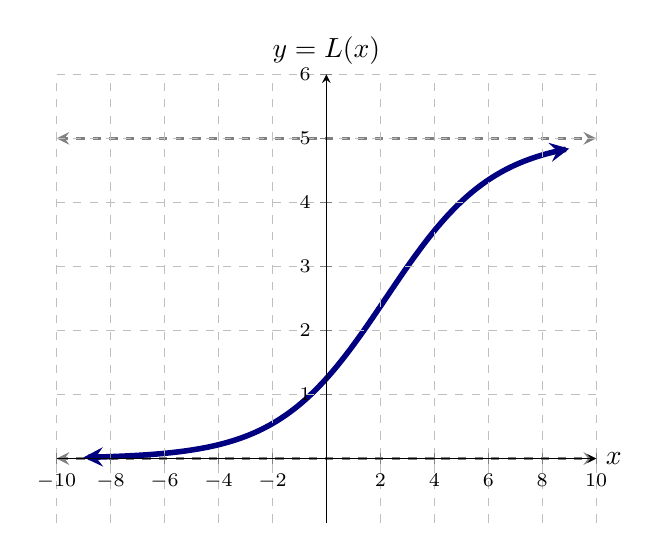
\begin{tikzpicture}
  \begin{axis}[
            domain=-10:10, ymax=6, xmax=10, ymin=-1, xmin=-10,
            axis lines =center, xlabel=$x$, ylabel={$y=L(x)$}, grid = major, grid style={dashed},
            ytick={1,2,3,4,5,6},
            xtick={-10,-8,-6,-4,-2,2,4,6,8,10},
            yticklabels={$1$,$2$,$3$,$4$,$5$,$6$}, 
            xticklabels={$-10$,$-8$,$-6$,$-4$,$-2$,$2$,$4$,$6$,$8$,$10$},
            ticklabel style={font=\scriptsize},
            every axis y label/.style={at=(current axis.above origin),anchor=south},
            every axis x label/.style={at=(current axis.right of origin),anchor=west},
            axis on top
          ]
          
          \addplot [line width=1, gray, dashed,samples=100,domain=(-10:10),<->] {5};
          \addplot [line width=1, gray, dashed,samples=100,domain=(-10:10),<->] {0};

            %\addplot [line width=2, penColor, smooth,samples=100,domain=(-9:9)] {5/(1 + 3 * e^(-x/2))};
          \addplot [line width=2, penColor, smooth,samples=100,domain=(-9:9),<->] {5/(1 + 3 * 2.7182^(-x/2))};

           




           

  \end{axis}
\end{tikzpicture}
\end{image}









$\blacktriangleright$ \textbf{Extrema:}  $L(x)$ has no global maximums or minimums, since it is a strictly increasing function.  


Could it wiggle slightly in the middle and cause a bump in the graph? Perhaps. Perhaps, there is a bump in the graph that we cannot see at our magnification.

If there was a bump in the graph, then there would be a top-of-the-bump point.  On either side of the top point the other points would be lower on the graph.  Then the graph moves downhill to the right from the top point, which would say the function is decreasing there.  But, we know $L$ is strictly increasing.  So, there can be no bumps.  $L$ has no local extrema.


This is not the end of the story. There could be a flat point, like on the graph of $y = x^3$. So, there could be a critical number still.  It doesn't look like it from the graph. But, perhaps the magnification provided by our graph is just too small to see it.



\end{example}





\section*{with Calculus}


Calculus will give us a formula for the derivative.

\[  L'(x) =   \frac{-15}{2} \cdot \frac{e^{-\tfrac{x}{2}}}{\left(1+3 e^{-\tfrac{x}{2}}\right)^2}    \]


This derivative has no zeros, which tells us that $L(x)$ has no critical numbers.  $L'(x)$ is always positive, which tells us that $L(x)$ is always increasing.












\begin{center}
\textbf{\textcolor{green!50!black}{ooooo-=-=-=-ooOoo-=-=-=-ooooo}} \\

more examples can be found by following this link\\ \link[More Examples of Analyzing Functions]{https://ximera.osu.edu/csccmathematics/precalculus2/precalculus2/analyzingFunctions/examples/exampleList}

\end{center}








\end{document}
